% =====================================================================
% From board to graph: a grid-based world model for hybrid human-AI role-play
% Target: Play4Change 2027 award, category C (Scientific Research).
% The call asks for an anonymous PDF (full text), an abstract of at most
% 1,800 characters and at most 3 keywords, typed into the form (see README).
% References: APA 7 via biblatex-apa (same .bib as the companion article).
% =====================================================================
\documentclass[11pt]{article}

\usepackage[utf8]{inputenc}
\usepackage[T1]{fontenc}
\usepackage[english]{babel}
\usepackage{csquotes}
\usepackage{mathptmx}
\usepackage[a4paper,margin=2.5cm]{geometry}
\usepackage{setspace}\setstretch{1.15}
\usepackage{amsmath,amssymb}
\usepackage{graphicx}
\usepackage{booktabs}
\usepackage{tabularx}
\usepackage{makecell}
\usepackage{xcolor}
\usepackage{tikz}
\usetikzlibrary{positioning,arrows.meta,calc,fit,backgrounds}
\usepackage[hidelinks]{hyperref}
\usepackage[style=apa,backend=biber]{biblatex}
\addbibresource{referencias.bib}

\graphicspath{{figuras/}}

\definecolor{lugar}{HTML}{CDE2FB}
\definecolor{atrator}{HTML}{F6C9B5}
\definecolor{tinta}{HTML}{3B3B38}
\definecolor{azul}{HTML}{2A78D6}
\definecolor{laranja}{HTML}{EB6834}

\newcommand{\R}{\mathbb{R}}

\title{\textbf{From Board to Graph: A Grid-Based World Model for Hybrid Human--AI Role-Play that Makes Narrative Power Visible}}
\author{[Anonymised for review]}
\date{}

\begin{document}
\maketitle

\begin{abstract}
\noindent
Whose story becomes the story of a community depends on who is where, who
knows what and who controls the places everyone needs. Games can make these
forces tangible. We present the design of a world model for role-playing in
which the world is a board, represented as a matrix, and in which human
players and generative-AI characters can share the same table. The model
connects three graphs: the spatial graph of the board, the temporal graph of
encounters between characters and the causal graph of the events they
produce. A character can only build on events it witnessed or heard about,
so the board decides which stories can meet. The design responds to an
empirical finding: when language-model agents share an unrestricted world,
their storylines merge into a single story within days, pulled by
\enquote{attractors} written into the premises. A proof of concept with
synthetic agents shows that space and information alone only delay this
convergence, that attractor places decide where it happens, and that two
simple mechanics, world-event cards and a focus rule, keep several stories
alive. We describe a physical kit in which causal links are drawn with yarn
between event cards, the hybrid human--AI protocol, and a research plan to
test whether playing on such a board helps groups see how space, information
and power shape the stories a community ends up telling.
\end{abstract}

% ---------------------------------------------------------------------
\section{Introduction}
% ---------------------------------------------------------------------

Every community tells itself stories about what happened: who was
responsible for a death, why the grain ran out, who is to blame for the debt.
Which of those stories survive is rarely a matter of truth alone. It depends
on who was present, on who heard what from whom, and on who controls the
places where people meet: the warehouse, the customs house, the mill.
Stories told by people at the periphery of these networks are absorbed into
the dominant account or never reach it. Games for social change aim to make
such processes experienceable, so that players can reflect on them
\parencite{flanagan2009,flanagan2014,bogost2007}.

Role-playing games are a natural medium for this. Their stories emerge from
what the participants do in a shared world \parencite{fine1983,montola2008},
and they are already used to develop perspective-taking and collaborative
skills \parencite{bowman2010,daniau2016}. Generative AI now makes it possible
to populate these worlds with artificial characters \parencite{park2023} and
to mix human and AI players at the same table. This raises a design
question with a social side: when humans and AI characters co-create a
community's story, what decides which stories survive?

A companion study, currently under review, gives a first answer for the
case in which every character is an AI agent. Language-model agents acting
freely in a small town produced four to five storylines on the second day of
play, and within a few days these storylines merged into one. Storylines
almost never ended; they were absorbed. The path of the convergence was not
random: the first fusions joined characters whose premises (their
objectives, secrets and beliefs) already referred to each other, and they
happened in the places those premises named. We call such premises and
places \emph{attractors}, borrowing the concept from dynamical systems
\parencite{strogatz2015}. One feature of that simulator matters here: a single
model call decided what every character did and saw everything that had
happened recently. The characters were, in effect, omniscient.

This paper takes the next step on the design side. We propose a world model
in which the world is a \emph{board}, with the properties that board games
make explicit: positions, distances, paths, regions and limited vision
\parencite{woods2012,salen2004}. On this board, a character only knows what
it saw or was told, and can only build on what it knows. The board is
represented as a matrix, and its structure propagates, through two other
graphs, to the structure of the story. The same board can be played by AI
agents in a simulator and by people with a physical kit, which allows human,
AI and hybrid tables to be compared with the same instruments.

The contributions are: (1) a formal model linking the board, the encounters
between characters and the causal graph of the story; (2) a proof of concept
with synthetic agents that identifies which board mechanics change
convergence and which do not; (3) a physical kit and a hybrid human--AI
protocol; and (4) a research plan, framed as a game for critical thinking
about how communities come to share one version of events.

% ---------------------------------------------------------------------
\section{Background}
% ---------------------------------------------------------------------

\paragraph{Space as narrative architecture.} Game spaces tell stories by
arranging places, paths and obstacles that channel movement and encounters
\parencite{jenkins2004}. A game's fiction is constrained by its rules, and
its rules are often spatial \parencite{juul2005,salen2004}. Modern board
games make these structures particularly legible: the map is visible to
everyone, and distances and adjacencies are part of the rules
\parencite{woods2012}. Architecture offers a precedent for measuring this:
space syntax describes buildings and cities as graphs and shows that the
position of a space in that graph predicts how much it is used and how
people meet in it \parencite{hillier1984}.

\paragraph{Grids as models of social dynamics.} Grids have a long history as
minimal models of social processes. Schelling's model showed that mild
individual preferences on a grid produce strong segregation
\parencite{schelling1971}; Sugarscape grew whole artificial societies on a
grid of resources \parencite{epstein1996}; cellular automata showed how local
rules on a lattice produce complex global patterns \parencite{wolfram1984}.
These models are also games in a loose sense, and they have been used to
teach exactly the point we care about: that collective outcomes can emerge
from local structure without anyone intending them.

\paragraph{Stories as graphs.} Narrative comprehension can be modelled as a
causal network of events \parencite{trabasso1985}, and the kernels of a plot
are the events with causal antecedents and consequences
\parencite{barthes1975,chatman1978}. Network science supplies the tools to
read such graphs: connected components, bridges and articulation points
\parencite{tarjan1972}, communities \parencite{blondel2008} and the
conditions under which a growing random graph becomes connected
\parencite{newman2018}. Emergent narrative research has long noted that
autonomous agents produce events more easily than stories with shape
\parencite{aylett1999,louchart2004,riedl2013}.

% ---------------------------------------------------------------------
\section{The model}
% ---------------------------------------------------------------------

\subsection{The board as a matrix}

The board is a grid of $n \times n$ cells. Each cell is a passage, a barrier
or part of a \emph{place}; a place $p$ is a connected region of cells with a
name and a description (the warehouse, the customs house, the chapel).
Figure~\ref{fig:tabuleiro} shows an example. Two non-barrier cells are
adjacent when they share a side (the 4-neighbourhood; hexagonal and
8-neighbour boards fit the same framework). The board is therefore a graph
$S = (C, A)$ whose vertices are the cells, and it is fully described by its
adjacency matrix $A \in \{0,1\}^{|C| \times |C|}$, with $A_{xy} = 1$ when
cells $x$ and $y$ are adjacent.

Matrix powers answer the board's basic questions. A cell $y$ is reachable
from $x$ in at most $k$ steps when
\begin{equation}
  \bigl[(I + A)^k\bigr]_{xy} > 0,
\end{equation}
so a character that moves $m$ cells per turn can reach, in one turn, the
cells in the support of row $x$ of $(I+A)^m$. Perception uses the same
operator: a character at $x$ with perception radius $\rho$ sees what happens
in the cells $V_\rho(x) = \{ y : [(I + A)^\rho]_{xy} > 0 \}$. Distances,
bottlenecks and chokepoints are properties of $S$: a bridge of $S$ is a
passage whose removal disconnects the board, and an articulation cell is a
cell whose removal does so \parencite{tarjan1972}. The places that many
premises mention are the \emph{attractor places}; their \emph{spatial basin}
is the set of cells from which characters tend to move toward them.

\begin{figure}[t]
\centering
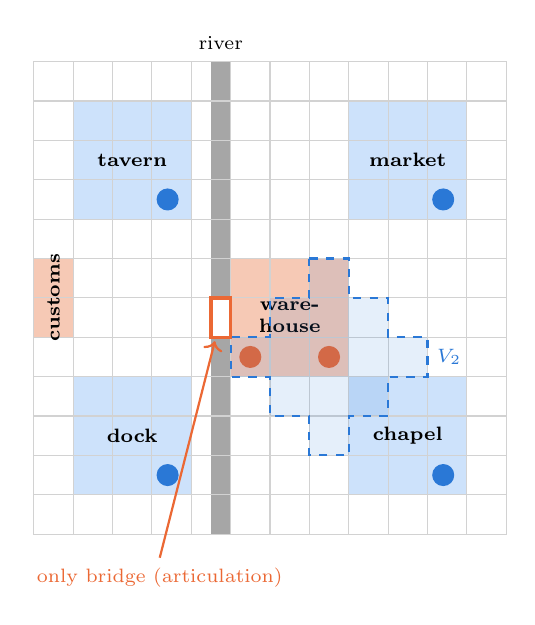
\begin{tikzpicture}[scale=0.5]
  % grade
  \foreach \x in {0,...,11} \foreach \y in {0,...,11} \draw[gray!35] (\x,\y) rectangle ++(1,1);
  % lugares (regiões)
  \newcommand{\regiao}[5]{\fill[#5] (#1,#2) rectangle (#3,#4);}
  \regiao{1}{1}{4}{4}{lugar}     % A
  \regiao{1}{8}{4}{11}{lugar}    % B
  \regiao{5}{4}{8}{7}{atrator}   % C (atrator)
  \regiao{8}{1}{11}{4}{lugar}    % D
  \regiao{8}{8}{11}{11}{lugar}   % E
  \regiao{0}{5}{1}{7}{atrator}   % F
  % barreira (rio) com uma ponte
  \foreach \y in {0,...,11} {\ifnum\y=5\else\fill[gray!70] (4.5,\y) rectangle ++(0.5,1);\fi}
  \foreach \x in {0,...,11} \foreach \y in {0,...,11} \draw[gray!35] (\x,\y) rectangle ++(1,1);
  \node[font=\scriptsize\bfseries] at (2.5,2.5) {dock};
  \node[font=\scriptsize\bfseries] at (2.5,9.5) {tavern};
  \node[font=\scriptsize\bfseries,align=center] at (6.5,5.5) {ware-\\house};
  \node[font=\scriptsize\bfseries] at (9.5,2.5) {chapel};
  \node[font=\scriptsize\bfseries] at (9.5,9.5) {market};
  \node[font=\scriptsize\bfseries,rotate=90] at (0.5,6) {customs};
  % ponte
  \draw[very thick,laranja] (4.5,5) rectangle (5,6);
  \node[font=\scriptsize,anchor=south] at (4.75,12.05) {river};
  \draw[->,laranja,thick] (3.2,-0.6) node[below,font=\scriptsize]{only bridge (articulation)} -- (4.6,4.9);
  % fichas
  \foreach \p/\c in {{3.4,1.5}/azul,{10.4,8.5}/azul,{5.5,4.5}/laranja,{7.5,4.5}/laranja,{10.4,1.5}/azul,{3.4,8.5}/azul}
    \fill[\c] (\p) circle (0.28);
  % raio de percepção de uma ficha (casa da ficha: (7,4))
  \foreach \dx in {-2,...,2} \foreach \dy in {-2,...,2} {
    \pgfmathtruncatemacro{\m}{abs(\dx)+abs(\dy)}
    \ifnum\m<3 \fill[azul,opacity=0.12] (7+\dx,4+\dy) rectangle ++(1,1); \fi}
  \draw[azul,thick,dashed] (7,7)--(8,7)--(8,6)--(9,6)--(9,5)--(10,5)--(10,4)--(9,4)--(9,3)--(8,3)--(8,2)--(7,2)--(7,3)--(6,3)--(6,4)--(5,4)--(5,5)--(6,5)--(6,6)--(7,6)--cycle;
  \node[font=\scriptsize,azul,anchor=west] at (10,4.5) {$V_2$};
\end{tikzpicture}
\caption{An example board: places are regions of cells; the warehouse and
the customs house are attractor places, named in several premises; a river
with a single bridge creates an articulation cell. Discs are characters;
the shaded cells are what one character sees with perception radius 2 (cells at most two steps away).}
\label{fig:tabuleiro}
\end{figure}

\subsection{Characters, encounters and knowledge}

Each character $a$ has a position $x_a(t)$ at turn $t$, a home place, and
premises: an objective, a secret and beliefs, as in the companion study.
Characters move toward the places their premises make relevant. Two
characters \emph{meet} at turn $t$ when one is within the other's perception
radius. Encounters form a temporal graph $H$ over the characters: let
$M^{(t)} \in \{0,1\}^{|\mathcal{A}| \times |\mathcal{A}|}$ be the encounter
matrix at turn $t$. Information can travel from $a$ to $b$ between turns
$t_0$ and $t_1$ only along a time-respecting path, which exists when
\begin{equation}
  \Bigl[\,\prod_{t = t_0}^{t_1 - 1} \bigl(I + M^{(t)}\bigr)\Bigr]_{ab} > 0,
\end{equation}
where the product is taken in Boolean arithmetic. Each character holds a
\emph{knowledge set} $K_a(t)$: the events it caused, the events it saw (those
in $V_\rho(x_a)$) and the events it heard about from characters it met, each
passed on with a rumour probability $\pi$.

\subsection{Events and the causal graph}

Each turn, each character acts. The action becomes an event $v$ with an
author, a cell, a turn and a list of declared causes, exactly as in the
existing simulator. The constraint that defines the model is
\begin{equation}
  u \in \mathrm{causes}(v) \;\Rightarrow\; u \in K_{\mathrm{author}(v)}\bigl(t(v)\bigr),
\end{equation}
that is, a character can only build on what it knows. For AI characters the
constraint is enforced by construction: each character is prompted
separately and the prompt lists only its knowledge set, instead of the single
omniscient call used so far. For human players it is enforced by the
physical kit (Section~\ref{sec:kit}).

The causal graph $G$ is built from the declared causes, and storylines are
its connected components, recomputed every day, with births, fusions and
closures tracked as in the companion study. The three graphs are nested:
$S$ bounds $H$ (characters can only meet where the board lets them go), and
$H$ bounds $G$ (an event can only cite another if information about it could
have travelled to its author). This yields design predictions that can be
read directly off the board. Attractor places should concentrate the
fusions; bridges and articulation cells of $S$ should be where separate
storylines first meet; and storylines rooted far apart on the board should
merge later. Figure~\ref{fig:camadas} summarises the three layers.

\begin{figure}[t]
\centering
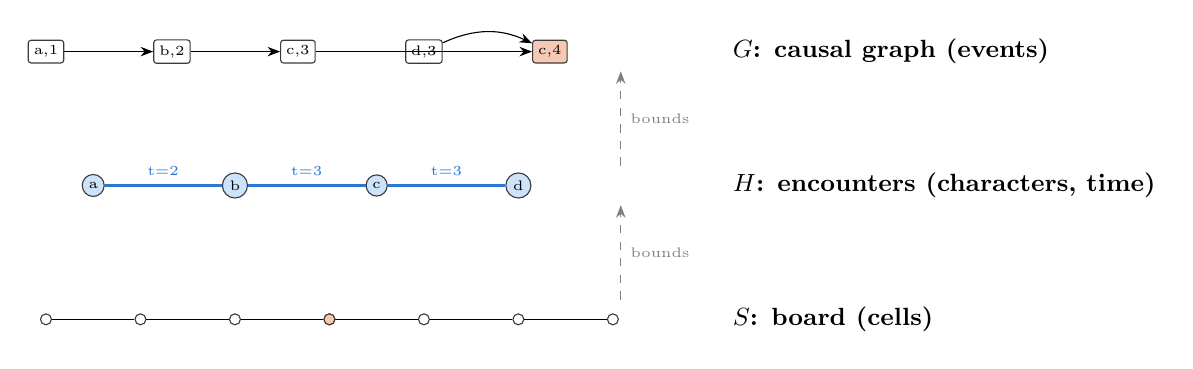
\begin{tikzpicture}[
  no/.style={circle,draw=tinta,fill=white,inner sep=1.4pt},
  ev/.style={rectangle,rounded corners=1pt,draw=tinta,fill=white,inner sep=2pt,font=\tiny},
  cam/.style={font=\small\bfseries,anchor=west},
  >={Stealth[length=1.6mm]}]
  % camada 1: espaço
  \begin{scope}[yshift=0cm]
    \foreach \i in {0,...,6} \node[no] (s\i) at (\i*1.2,0) {};
    \foreach \i [evaluate=\i as \j using int(\i+1)] in {0,...,5} \draw (s\i) -- (s\j);
    \node[no,fill=atrator] at (s3) {};
    \node[cam] at (8.6,0) {$S$: board (cells)};
  \end{scope}
  % camada 2: encontros
  \begin{scope}[yshift=1.7cm]
    \foreach \i/\x in {a/0.6,b/2.4,c/4.2,d/6.0} \node[no,fill=lugar] (h\i) at (\x,0) {\tiny\i};
    \draw[azul,thick] (ha) -- node[above,font=\tiny]{t=2} (hb);
    \draw[azul,thick] (hb) -- node[above,font=\tiny]{t=3} (hc);
    \draw[azul,thick] (hc) -- node[above,font=\tiny]{t=3} (hd);
    \node[cam] at (8.6,0) {$H$: encounters (characters, time)};
  \end{scope}
  % camada 3: eventos
  \begin{scope}[yshift=3.4cm]
    \node[ev] (e1) at (0,0) {a,1};
    \node[ev] (e2) at (1.6,0) {b,2};
    \node[ev] (e3) at (3.2,0) {c,3};
    \node[ev] (e4) at (4.8,0) {d,3};
    \node[ev,fill=atrator] (e5) at (6.4,0) {c,4};
    \draw[->] (e1) -- (e2);
    \draw[->] (e2) -- (e3);
    \draw[->,bend left=25] (e4) to (e5);
    \draw[->] (e3) -- (e5);
    \node[cam] at (8.6,0) {$G$: causal graph (events)};
  \end{scope}
  \draw[->,gray,dashed] (7.3,0.25) -- node[right,font=\tiny,text=gray]{bounds} (7.3,1.45);
  \draw[->,gray,dashed] (7.3,1.95) -- node[right,font=\tiny,text=gray]{bounds} (7.3,3.15);
\end{tikzpicture}
\caption{The three layers. Where characters can go ($S$) bounds whom they
meet and when ($H$), which bounds what each event can cite ($G$). The
highlighted event, at an attractor place, merges two storylines.}
\label{fig:camadas}
\end{figure}

% ---------------------------------------------------------------------
\section{Proof of concept with synthetic agents}
% ---------------------------------------------------------------------

Before involving language models or people, we asked which board mechanics
can change convergence at all. We wrote a minimal simulation in which six
synthetic characters move on a $12 \times 12$ board with six places, two of
them attractor places, and act once per day for 20 days. Each event cites a
number of causes drawn from the distribution observed with language-model
agents in the companion study (mostly one or two causes; almost never none),
chosen at random among the recent events the author \emph{knows}. The
characters have no content and no intentions: what is tested is the
structure alone. We compared the omniscient regime of the existing simulator
with board regimes that vary the perception radius, rumours and attractor
places, and with two design levers: \emph{event cards}, two world events per
day that appear in random cells with no cause, and a \emph{focus rule}, under
which, in 80\% of actions, all causes must come from the same storyline.
Each condition was run 500 times; the script is in the repository.

\begin{figure}[t]
\centering
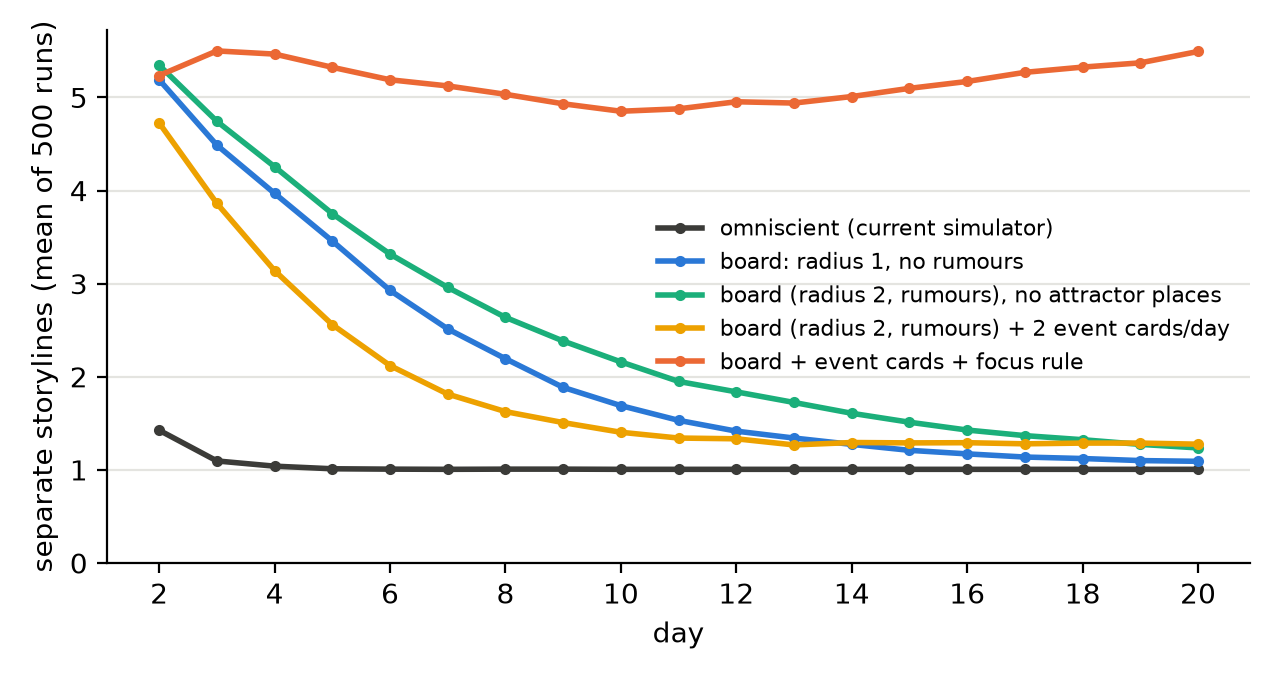
\includegraphics[width=0.8\textwidth]{linhas_por_condicao.png}
\caption{Separate storylines per day in the synthetic proof of concept (mean
of 500 runs per condition, 20 days).}
\label{fig:prova}
\end{figure}

\begin{table}[t]
\centering\small
\caption{Proof of concept, 20 days, 500 runs per condition.}
\label{tab:prova}
\begin{tabularx}{\textwidth}{@{}Xrrrr@{}}
\toprule
Condition & \makecell{Storylines\\at the end} & \makecell{Runs ending\\with one} & \makecell{Born after\\day 2} & \makecell{Fusions near\\attractors} \\
\midrule
Omniscient (current simulator) & 1.01 & 99\% & 0.1 & 91\% \\
Board, radius 2, rumours & 1.05 & 95\% & 0.0 & 85\% \\
Board, radius 1, no rumours & 1.09 & 91\% & 0.0 & 85\% \\
Board, radius 2, rumours, no attractor places & 1.24 & 79\% & 0.0 & 66\% \\
Board + 2 event cards per day & 1.28 & 76\% & 1.3 & 86\% \\
Board + event cards + focus rule & 5.49 & 2\% & 6.0 & 84\% \\
\bottomrule
\end{tabularx}
\end{table}

Three results stand out (Figure~\ref{fig:prova}, Table~\ref{tab:prova}).
First, \emph{information changes the beginning, not the end}. In the
omniscient regime, the actions of the second day already cite each other
across characters and only 1.5 storylines are born on average; on the board,
each character mostly knows its own past, and about five storylines are
born, the same order observed with language-model agents. But on every
board without further mechanics, almost all runs still end with a single
storyline. Reducing the perception radius or removing rumours only slows the
process.

Second, \emph{attractor places decide where, and partly whether}. With
attractor places, more than 80\% of fusions happen next to them; without
them, the share falls to 66\% and one run in five keeps more than one
storyline.

Third, \emph{new stories need new seeds and a reason not to knot}. Since
every character always knows its own past and almost always cites
something, no storyline is born after the second day unless the world
supplies events without causes. Event cards provide such seeds, but alone
they are soon absorbed. Combined with the focus rule, which keeps an action
inside one storyline, they sustain five to six storylines throughout the
session, with new ones being born as others merge.

The proof of concept has obvious limits: synthetic characters choose at
random and have no premises in the textual sense. Its value is to separate
what the board can do from what content does, and to point at the
mechanics worth testing with people and language models.

% ---------------------------------------------------------------------
\section{The physical kit and the hybrid protocol}
\label{sec:kit}
% ---------------------------------------------------------------------

The same board is printed for a table of four to eight participants. The kit
has: the board, with places and a river; one token and one character sheet
per character, with objective, secret and beliefs; blank \emph{event cards},
on which a player writes what the character does, the turn and the identifier
of each cause; coloured yarn, which connects each event card to the cards it
cites; a deck of world-event cards; and screens that hide each player's
known cards.

A turn has four steps. (1) Characters move up to $m$ cells. (2) The
facilitator reveals world-event cards in the drawn cells. (3) Each player
writes an event card and places it on the cell where it happens; the card's
causes must be cards the character knows, and the facilitator ties the yarn.
(4) Knowledge is updated: a player adds to their hand the cards placed within
the perception radius of their token, and players whose tokens meet may show
each other cards from their hands (rumours). Optional rules switch the focus
rule on or off, or change $\rho$ and the number of world-event cards.

In hybrid tables, some characters are played by the simulator. The
facilitator, or a companion app, enters the AI characters' positions and
known cards; the simulator, prompted per character with only that
knowledge, returns the action and its causes, which are written on cards
like any other. Because every event card carries the same fields as the
simulator's event log, a photographed or transcribed table yields the same
data as a simulated session, and all analyses (storylines, fusions,
attractors) run unchanged on human, AI and hybrid tables.

At the end of a session the yarn \emph{is} the causal graph. The debrief uses
it directly: which storylines merged, at which card, in which place; which
characters' storylines were absorbed into others and never had their own
ending; who knew what, and when.

% ---------------------------------------------------------------------
\section{Research plan}
% ---------------------------------------------------------------------

We plan two studies, to be pre-registered with the same procedures as the
companion study \parencite{nosek2018}.

\emph{Study 1 (simulation with language-model agents).} The existing
simulator will be extended with the board and with per-character prompts
restricted to knowledge sets. With the same worlds and models as the
companion study, we will cross the omniscient and board regimes, the
perception radius, rumours, event cards and the focus rule. Hypotheses:
(H1) on the board, more storylines are born and fusions happen later than in
the omniscient regime; (H2) fusions concentrate in attractor places and at
articulation cells of the board; (H3) without event cards, no storylines are
born after the first days in any regime; (H4) event cards with the focus rule
sustain several storylines and allow closures by stability.

\emph{Study 2 (tables with people).} Workshops with groups of students and
community participants will play the same scenario in three formats: human
only, AI only (projected) and hybrid. Each group plays twice, with and
without the board constraints. Measures include the same graph metrics,
plus a short post-game reflection in which participants describe how the
town's story was formed and who shaped it, coded for references to
information, place and power. (H5) Human tables cite fewer causes per event
than AI agents and keep more storylines separate; (H6) after the debrief
with the yarn graph, participants refer more often to structural factors
(who knew what, who controlled which place) when explaining the outcome of
the story. Studies with people will follow the ethics procedures of the
authors' institution, with informed consent and anonymised data.

% ---------------------------------------------------------------------
\section{Relevance for social change}
% ---------------------------------------------------------------------

The board is a small model of a social question: how a community comes to
share one version of events. In the companion study, the story converged
around the places and secrets the world's authors had entangled; in this
model, the same happens around places that control movement and around
characters who meet many others. Players who see their character's
storyline absorbed into someone else's, because they were on the wrong side
of the river or never heard the rumour, experience, rather than are told,
how access to information and to central places translates into narrative
power. The debrief makes that experience explicit with an object everyone
built together, the yarn graph.

This connects to three themes of games for social change. \emph{Critical
thinking}: the game asks why a story became the story, not only what
happened. \emph{Civic awareness}: the scenarios (a harbour town with debt,
bribery and smuggling; a village rationing grain before winter) are about
commons, corruption and scarcity, and the board shows how place and
information shape collective decisions about them. \emph{Inclusion}: the
mechanics show how peripheral voices are absorbed, and the levers that
change it (event cards that seed new stories, a focus rule that protects a
thread, more bridges across the river) are design choices players can
discuss and change. Because the same board is played by AI characters, it
also opens a conversation about how generative AI, which in our data links
everything it sees, may amplify the convergence toward a single account.

% ---------------------------------------------------------------------
\section{Limitations and next steps}
% ---------------------------------------------------------------------

The model is a design proposal with a proof of concept, not an evaluated
game. The proof of concept uses synthetic characters and says nothing about
the content language models or people would produce on the board. The
formal model treats knowledge as sets of events, which is a simplification of
what characters believe and misremember. The physical kit has not yet been
playtested; its turn structure may be too heavy for some groups, and a
digital companion may be needed to manage knowledge sets. The next steps are
the board module of the simulator, a first playtest of the kit, and the
pre-registration of the two studies.

% ---------------------------------------------------------------------
\section{Conclusion}
% ---------------------------------------------------------------------

Representing the world of a role-playing game as a board, and the board as a
matrix, makes it possible to reason about the story with the tools of graph
theory: the board bounds the encounters, the encounters bound the causal
graph, and the causal graph is the story. A proof of concept shows that the
board alone does not prevent a shared story from collapsing into one, that
attractor places decide where it collapses, and that two simple mechanics
keep several stories alive. The same board, played by people and AI
characters with yarn and cards, turns this structure into something a group
can see and discuss: how space, information and power decide which story a
community ends up telling.

\printbibliography

\end{document}
